\documentclass[a4paper,12pt]{article}
\usepackage[margin=1in]{geometry}

\usepackage[T2A]{fontenc}			% кодировка
\usepackage[utf8]{inputenc}			% кодировка исходного текста
\usepackage[english,russian]{babel}	% локализация и переносы
\usepackage{graphicx}                % Математика
\usepackage{amsmath,amsfonts,amssymb,amsthm,mathtools} 
\usepackage{mathtext}
\usepackage[T2A]{fontenc}
\usepackage[utf8]{inputenc}

\usepackage{wasysym}

%Заговолок
\author{Бичина Марина 
группа Б04-005 1 курса ФЭФМ}
\title{}
\date{}


\begin{document} % начало документа

\begin{center}
\begin{Large}
{Бичина Марина Б04-005, Лабораторная работа № 5.1.2 <<Исследование эффекта Комптона>>}
\end{Large}
\end{center}
\paragraph{Цель работы:} 
\begin{enumerate}
\itemsep0em
\item Исследовать энергетический спектр $\gamma$ квантов, рассеянных на графите
\item Определить энергию рассеянных $\gamma$ квантов в зависимости от угла рассеяния $\theta$
\item Определить энергию покоя частиц, на которых происходит комптоновское рассеяние
\end{enumerate}
\paragraph{Оборудование:}
\begin{enumerate}
\itemsep0em
\item Сцинтилляционный спектрометр
\item Источник направленного $\gamma$--излучения
\item Графитовая мишень
\end{enumerate}


\paragraph{Теоретическая справка:}
\paragraph{}
\textbf{\textit{Эффект Комптона}} -- это увеличение длины волны рассеянного излучения по сравнению с падающим. Интерпретируется как результат упругого соударения $\gamma$-кванта (фотона) и свободного электрона. При исследовании данного эффекта, можно наблюдать проявление двойственной природы излучения. 

 В нашем случае $\gamma$--квант испускаемый цезием 137 рассеивается об электроны в графитовом цилиндре. Данный эффект не объясняется классической электродинамикой, для его объяснения необходимо считать взаимодействие фотона и электрона упругим соударением.

\paragraph{} Из расчёта абсолютно упругого соударения фотона и электрона, используя закон сохранения импульса и энергии получим формулу для изменения длины волны рассеянного $\gamma$--кванта:

\begin{equation}
\Delta \lambda = \lambda_1 - \lambda_0 = \frac{h}{mc}(1 - \cos{\theta}) = \Lambda_{K}(1 - \cos{\theta}), 
\label{e:e1}
\end{equation}

\noindent где $\Lambda_{K} = \frac{h}{mc} = 2.42 \cdot 10^{-10}$ см -- комптоновская длина волны электрона.

Подставив в формулу (\ref{e:e1}) энергию $\gamma$--кванта $\varepsilon = \hbar \omega$ получим другую форму записи:

\begin{equation}
\frac{1}{\varepsilon(\theta)} - \frac{1}{\varepsilon_0} = 1 - \cos{\theta}.
\label{e:e2}
\end{equation}
\paragraph{Описание установки:}
\paragraph{}
\begin{figure}[h!]
\centering
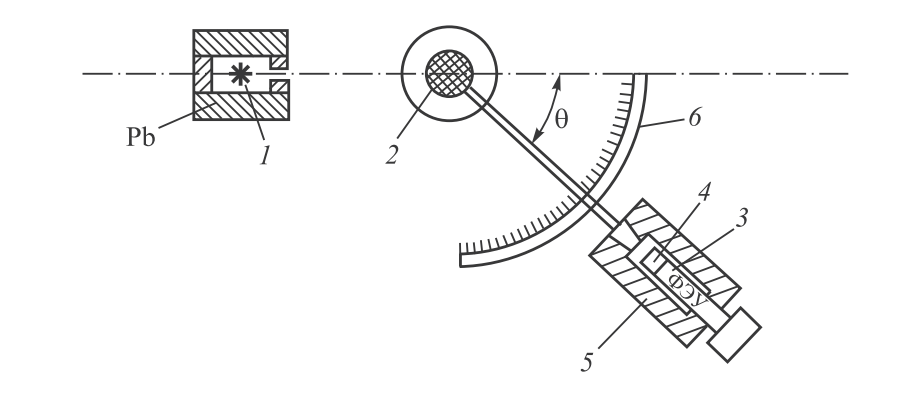
\includegraphics[scale=0.6]{setup.png}
\caption{Блок-схема установки по изучению рассеяния $\gamma$-квантов}
\end{figure} 

Элементы установки: 
\begin{enumerate}
\itemsep0em
\item Источник излучения $^{137}Cs$, испускающий $\gamma$-лучи с энергией 662 кэВ (помещен в свинцовый контейнер с коллиматором)
\item графитовая мишень размерами 40 мм х 100 мм
\\\\
Сцинтилляционный счетчик:

\item ФЭУ
\item сцинтиллятор (кристалл NaI диаметром 40 мм и высотой 40 мм)
\item  свинцовый коллиматор
\\
\item лимб
\end{enumerate}

Сцинтилляционный счетчик подключается к усилителю-анализатору, который фиксирует попадание $\gamma$-кванта в счетчик. Далее идет передача данных о его энергии на компьютер в 1024 дискретных уровнях (каналах), номере которых прямо пропорционален значению энергии. На экране компьютера выводится гистограмма, по оси абсцисс которой откладывается амплитуда анализируемого импульса (номер канала), а по оси ординат -- число импульсов заданной амплитуды (в данном канале).
\paragraph{Ход работы:}
\begin{enumerate}
\itemsep0em
\item  При помощи экспериментальной установки измерим зависимость номера фотопика $N$ от положения сцинтилляционного счётчика $\theta$. В качестве номера фотопика возьмём номер наибольшого столбца в гистограмме, соответствующего к пику созданным рассеянными фотонами.
\item Данные занесем в таблицу \ref{tab:data}.

\begin{table}[h!]
\centering
\begin{tabular}{|c|c|c|c|c|c|c|c|c|c|c|c|c|c|c|}
\hline
$\theta, ^o$ & 0   & 10  & 20  & 30  & 40  & 50  & 60  & 70  & 80  & 90  & 100 & 110 & 120 & 130 \\ \hline
$N$      & 897 & 893 & 845 & 689 & 683 & 560 & 488 & 421 & 383 & 345 & 313 & 280 & 261 & 246 \\ \hline
\end{tabular}
\caption{Значение угла в градусах и соответствующий фотопик.}
\label{tab:data}
\end{table}
Учитывая то, что номер канала фотопика прямо пропорционален энергии кванта зафиксированного счётчиком, заменим в формуле (\ref{e:e2}) энергию $\varepsilon$ номером канала максимума фотопика $N$, и добавив неизвестный коэффициент пропорциональности $A$, получим формулу:

\begin{equation}
\frac{1}{N(\theta)} - \frac{1}{N(0)} = A(1 - \cos{\theta}).
\label{e:e3}
\end{equation}

\item Для более удобной обработки измеренных данных (табл. \ref{tab:data}), построим график зависимости $1 - \cos{\theta}$ от $1/N(\theta)$, и проведём через полученные точки наилучшею прямую (по МНК) (рис. 2). 
\begin{figure}[h!]
\centering
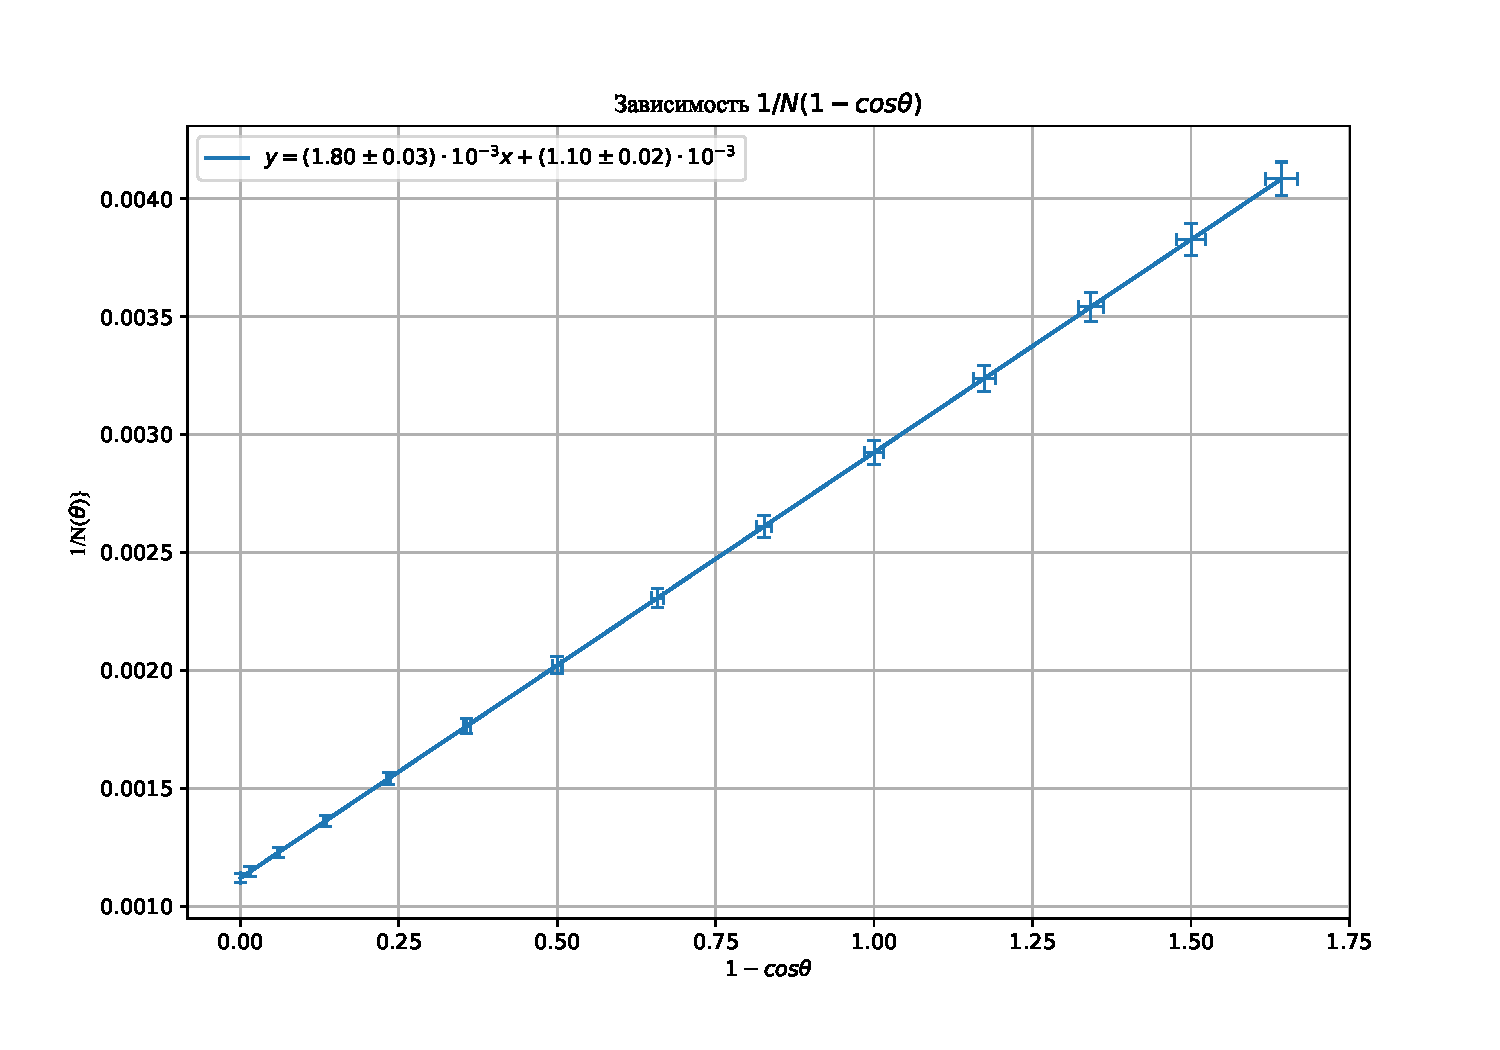
\includegraphics[scale=0.6]{plot_5_1_2 .pdf} 
\end{figure}

\item По наилучшей прямой определим наилучшие значения для $N$ при $\theta = 0^o$ и $\theta = 90^o$, получим:

\[
\theta = 0^o \; \Rightarrow \; x = 0 \; \Rightarrow y(0) = (1.12 \pm 0.02) \cdot 10^{-3},
\]\[
N(0) = \frac{1}{y(0)} = 893, \; \Delta N(0) = N(0) \cdot \frac{\Delta y(0)}{y(0)} = 16, \; N_\text{наил}(0) = 890 \pm 20;
\]\[
\theta = 90^o \; \Rightarrow \; x = 1 \; \Rightarrow y(1) = (2.92 \pm 0.04) \cdot 10^{-3},
\]\[
N(90) = \frac{1}{y(1)} = 342, \; \Delta N(90) = N(90) \cdot \frac{\Delta y(1)}{y(1)} = 5, \;
N_\text{наил}(90) = 342 \pm 5.
\]
\item Теперь проверим результаты:
\paragraph{} Воспользуемся формулой (\ref{e:e2}), подставив значение $\theta = 90^o$:

\[
mc^2 \left( \frac{1}{E(90)} - \frac{1}{E(0)} \right) = 1,
\]

\noindent или

\[
mc^2 = E(0)\frac{E(90)}{E(0) - E(90)} = E_\gamma \frac{N(90)}{N(0) - N(90)},
\]

\noindent где $E_\gamma$ -- энергия электронов, рассеянных вперёд, или просто энергии $\gamma$--лучей.

\item Теперь найдём энергию покоя частицы $E_\text{П} = mc^2$, рассчитанной по формуле:

\[
E_\text{П} = E_\gamma \frac{N_\text{наил}(90)}{N_\text{наил}(0) - N_\text{наил}(90)} = 662 \text{ кэВ} \cdot \frac{342}{890 - 342} = 413 \text{ кэВ},
\] \[
\Delta E_\text{П} = E_\text{П} \cdot \sqrt{2 \left( \frac{\Delta N(90)}{N(90)} \right)^2 + \left( \frac{\Delta N(0)}{N(0)} \right)^2} = 13 \text{ кэВ}.
\]

Получили $mc^2 = 410 \pm 20$ кэВ, что значительно ниже действительного значения $mc^2 = 511$ кэВ.
\end{enumerate}
\paragraph{Выводы:}
\begin{enumerate}
\item Пронаблюдали эффект Комптона при помощи сцинтилляционного счётчика, заметив изменение энергии рассеянных $\gamma$--квантов при изменении угла рассеяния.
\item Подтвердили состоятельность формулы (\ref{e:e1}) и её вывода, получив прямую зависимость на графике (рис. 2).
\item Посчитали энергию покоя электронов, рассеивающих $\gamma$--кванты, получив значение $mc^2 = 410 \pm 20$ кэВ, что на $20\%$ отличается от действительного значения $mc^2 = 511$ кэВ. Это различие можно объяснить неточностью при определении номера канала $N$, соответствующего фотопику.
\end{enumerate}
\end{document}